\section{Results}\label{sec:results}

\subsection{RQ1: accuracy of the statistical core}\label{sec:main}

\Cref{tab:main} and \cref{fig:main} report all arms on the 103 RCA100 cases. Without any language model, \core{} reaches a Final score
of 62.9 [57.4, 68.5]; it names the exact root entity in 64 cases, the exact type in 45 and both in 39, in 78\,s per incident on a
CPU. An LLM that decides from the same calibrated evidence (Evidence$\rightarrow$LLM, Qwen2.5-7B) reaches 42.7: the difference,
+20.2 [15.0, 25.6] ($p=2.8\times10^{-10}$; Final$_\text{step}$ +13.5, $p=1.2\times10^{-6}$), comes from the type (exact type 33 cases
for \core{} only versus 9 for the LLM only, McNemar $p=0.0003$), not from the entity (8 versus 10, $p=0.81$); given good evidence,
the 7B model localises as well as the computed belief (EL 71.8 versus 68.9) but types far worse (FI 20.4 versus 43.7). An LLM that
sees the alert only (Direct LLM) reaches 18.8 and never names the exact entity (\core{} $-$ Direct: +44.1 [38.0, 50.3],
$p=1.5\times10^{-17}$). The evidence thus explains about half of the gap between the alert-only LLM and \core{}, and the computed
belief the other half.

\begin{table}[!htbp]
\centering
\caption{Results on the 103 RCA100 cases (0--100; 95\% bootstrap CI). Final uses the headline RP, Final$_\text{step}$ the
step-anchored RP (\cref{sec:problem}). Exact: number of cases with the exact entity / type / both.}\label{tab:main}
\footnotesize
\setlength{\tabcolsep}{3pt}
\begin{tabular}{@{}lccccccc@{}}
\toprule
Arm & Final & Final$_\text{step}$ & EL & FI & RP & Exact \\
\midrule
\core{} (no LLM) & \textbf{62.9} [57.4, 68.5] & \textbf{56.2} [50.4, 61.9] & 68.9 & \textbf{43.7} & 74.1 & 64/45/39 \\
\core{} $-$\Mod{2} & 57.3 [52.0, 62.9] & 50.6 [45.0, 56.5] & 64.2 & 32.0 & 73.3 & 57/33/26 \\
\core{}+LLM, 7B & 59.2 [53.9, 64.6] & 52.5 [47.0, 58.1] & 66.5 & 35.0 & 73.7 & 60/36/30 \\
\core{}+LLM, 120B & 59.4 [54.0, 65.2] & 52.7 [47.1, 58.6] & 65.7 & 36.9 & 73.7 & 59/38/32 \\
Belief$\rightarrow$LLM, 7B & 48.0 [42.6, 53.6] & 48.0 [42.6, 53.6] & 67.9 & \textbf{43.7} & 25.8 & 63/45/39 \\
Evidence$\rightarrow$LLM, 7B & 42.7 [38.1, 47.4] & 42.7 [38.1, 47.4] & \textbf{71.8} & 20.4 & 26.2 & 66/21/18 \\
Direct LLM, 7B & 18.8 [15.3, 22.5] & 18.8 [15.3, 22.5] & 28.0 & 14.6 & 10.9 & 0/15/0 \\
\midrule
Evidence$\rightarrow$LLM, 120B & \pending{run} & & & & & \\
Belief$\rightarrow$LLM, 120B & \pending{run} & & & & & \\
\bottomrule
\end{tabular}
\begin{flushleft}\footnotesize 7B = Qwen2.5-7B-Instruct (local); 120B = gpt-oss-120b (API).\end{flushleft}
\end{table}

\begin{figure}[!htbp]
\centering
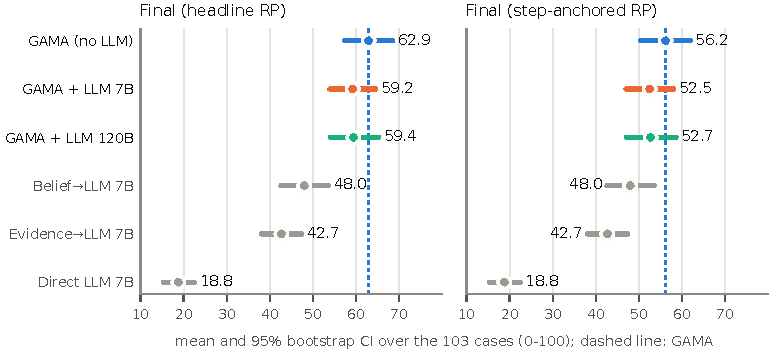
\includegraphics[width=\textwidth]{figs/fig2_main.pdf}
\caption{Final score of every arm on the 103 RCA100 cases with 95\% bootstrap intervals; left with the headline reasoning-process
score, right with the step-anchored one. The dashed line marks \core{}. Arms in which an LLM writes the chain return no evidence
items, so the retrieval-based half of the headline RP is zero for them; the step-anchored score compares chains on equal terms.}
\label{fig:main}
\end{figure}

\paragraph{By fault group}
\Cref{fig:groups} breaks EL and FI down by fault group. \core{} localises JVM-runtime faults perfectly and types 69\% of them;
resource and performance faults are typed in 80\% of the cases. Its weak spot is node faults (EL 22.3): a node fault slows every
service it hosts, and when the node's own CPU or memory signal does not stand out against its peers, a hosted service with strong
trace evidence wins. Middleware and database faults are localised (EL 77.9) but rarely typed (FI 23.1); plausibly because slow SQL and
database network latency look alike in spans when no database-side metrics are exported.

\begin{figure}[!htbp]
\centering
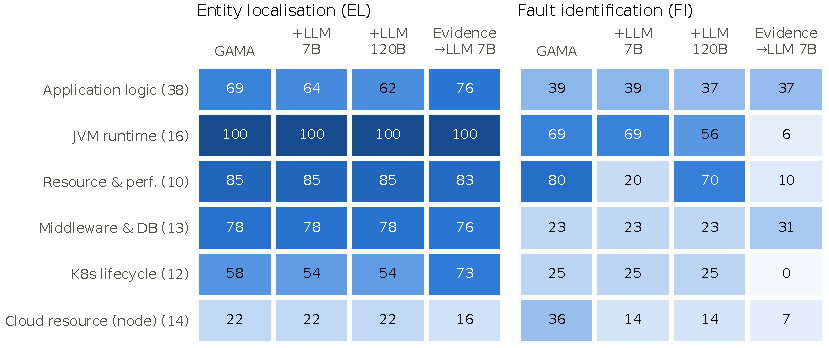
\includegraphics[width=\textwidth]{figs/fig3_groups.pdf}
\caption{Entity localisation (left) and fault identification (right) by RCA100 fault group, for \core{}, \core{} with the bounded LLM
(7B and 120B) and Evidence$\rightarrow$LLM (7B). Darker is better.}\label{fig:groups}
\end{figure}

\subsection{RQ2: contribution of the modules}\label{sec:ablation}

\Cref{tab:ablation} reports the leave-one-module-out runs. Removing trace-origin attribution (\Mod{2}) costs 5.6 Final points
[2.3, 9.3] ($p=0.009$; 18 cases better with the module, 5 worse): the module mainly identifies the \emph{type}
(exact type 14 : 2, McNemar $p=0.004$), because the messages and status codes of the origin spans name rate limiting, null pointers
and HTTP 5xx errors (application-logic FI 39.5 with the module versus 10.5 without). It costs node faults, however: node EL drops
from 33.9 to 22.3 with the module, since a node that hosts several origin services can lose to one of them, and a node without its
own signal can win on their strength. \pending{leave-one-out runs of \Mod{1}, \Mod{3}, \Mod{4}, \Mod{5} and \Mod{6}.}

\begin{table}[!htbp]
\centering
\caption{Leave-one-module-out ablation on the 103 RCA100 cases: change of the Final score when a module is removed from \core{}
(paired Wilcoxon, two-sided, Holm over the six modules), cases better / worse with the module, and McNemar counts for the exact
type (with : without).}\label{tab:ablation}
\footnotesize
\setlength{\tabcolsep}{4pt}
\begin{tabular}{@{}lcccc@{}}
\toprule
Module removed & $\Delta$Final [95\% CI] & $p$ & better / worse & exact type \\
\midrule
\Mod{1} corroboration & \tbd & \tbd & \tbd & \tbd \\
\Mod{2} trace origins & $-5.6$ [$-9.3$, $-2.3$] & 0.009$^\dagger$ & 18 / 5 & 14 : 2 \\
\Mod{3} mechanism typing & \tbd & \tbd & \tbd & \tbd \\
\Mod{4} load explain-away & \tbd & \tbd & \tbd & \tbd \\
\Mod{5} mechanism text & \tbd & \tbd & \tbd & \tbd \\
\Mod{6} cited chain (RP only) & \tbd & \tbd & \tbd & -- \\
\bottomrule
\end{tabular}
\begin{flushleft}\footnotesize $^\dagger$ unadjusted; the Holm adjustment is applied once all six runs are available.\end{flushleft}
\end{table}

\subsection{RQ3: what the language model adds}\label{sec:llmrole}

\paragraph{Decision}
With either backbone, the bounded LLM lowers the Final score of the statistical core (\cref{tab:llmtests}, \cref{fig:llm}a):
by 3.7 points with Qwen2.5-7B ($p=0.008$; 2 cases better, 14 worse) and by 3.5 points with gpt-oss-120b ($p=0.03$; 3 better, 13
worse). The two backbones end at the same score ($+0.2$, $p=0.62$). Two mechanisms are responsible (post-hoc analysis, no design
change). (i) \emph{Shortlist typing} changed the computed type in 25 (7B) and 21 (120B) cases; only 3 and 2 of these changes reached
the true type, while 10 and 7 replaced a correct type (\cref{fig:llm}b). The changes concentrate where the telemetry cannot separate
two types: the 7B model turned \emph{cpuFullLoad} into \emph{cpuDeadLoop} in seven cases; the 120B model avoided this pattern but
turned \emph{memoryPressure} into \emph{fullGC} in two; both models replaced node CPU faults by disk or memory faults (node FI 35.7
$\rightarrow$ 14.3). (ii) The \emph{text sensor} moved a correct entity away in four cases---the same four cases with both
backbones---which points to the weight of the sensor's answer in the likelihood rather than to the model.

\paragraph{The computed belief and a free LLM}
Given the posterior and full authority (Belief$\rightarrow$LLM), the 7B model kept \core{}'s entity and type in 102 of 103 cases
(the remaining case is a truncated answer that also repeated it): it defers to the computed belief (B1). The belief helps the LLM:
Belief$\rightarrow$LLM exceeds Evidence$\rightarrow$LLM by 5.3 points [0.2, 10.4] (one-sided $p=0.025$; exact type 33 : 9), confirming
B2. Compared with the bounded use of the same model (B3), the free LLM decides better (exact type 11 : 2), but its own chain is weaker
than the computed one (chain-node match 51.5 versus 72.7, step-anchored checkpoints 0.0 versus 0.307), so its Final$_\text{step}$ is
4.4 points lower.

\paragraph{Explanation}
Scale changes the explanation, not the decision (\cref{fig:llm}c). The narrator of gpt-oss-120b satisfies 0.284 of the step-anchored
evidence checkpoints against 0.107 for the 7B narrator on the same cases (51 cases higher, 5 lower; one-sided Wilcoxon
$p=2\times10^{-10}$), close to the computed chain (0.307); 88\% of the numbers it quotes appear in the evidence (7B: 92\%). This
supports H3.

\begin{figure}[!htbp]
\centering
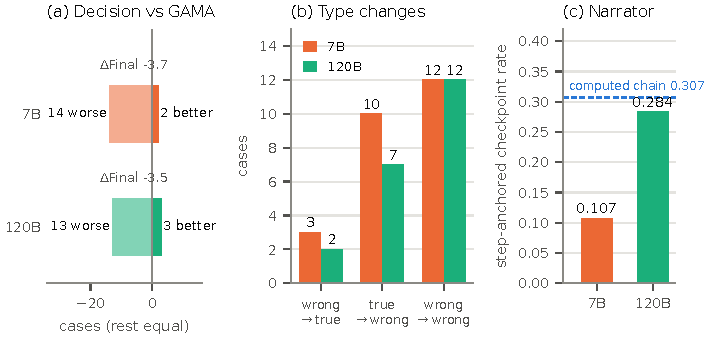
\includegraphics[width=\textwidth]{figs/fig4_llm.pdf}
\caption{What the bounded LLM adds. (a) Cases in which \core{} + LLM scores better or worse than \core{} (the remaining cases are
equal). (b) Changes of the computed type made by shortlist typing. (c) Step-anchored checkpoint rate of the LLM narrator; the dashed
line is the chain computed by \Mod{6}.}\label{fig:llm}
\end{figure}

\begin{table}[!htbp]
\centering
\caption{Pre-registered comparisons and hypotheses on the 103 RCA100 cases. $\Delta$ is the paired difference of Final scores
(first minus second) with 95\% bootstrap CI; $p$ from the Wilcoxon signed-rank test (Holm within family).}\label{tab:llmtests}
\footnotesize
\setlength{\tabcolsep}{3pt}
\begin{tabularx}{\textwidth}{@{}>{\raggedright\arraybackslash}X ccc>{\raggedright\arraybackslash}p{2.4cm}@{}}
\toprule
Comparison & $\Delta$Final [95\% CI] & $\Delta$Final$_\text{step}$ & $p$ & Outcome \\
\midrule
\core{} vs Evidence$\rightarrow$LLM (7B) & $+20.2$ [15.0, 25.6] & $+13.5$ & $2.8\times10^{-10}$ & structure wins \\
\core{}+LLM (7B) vs \core{} & $-3.7$ [$-6.4$, $-1.4$] & $-3.7$ & 0.008 & LLM lowers the score \\
\core{}+LLM (120B) vs \core{} & $-3.5$ [$-6.3$, $-0.9$] & $-3.5$ & 0.03 & LLM lowers the score \\
\core{}+LLM (120B) vs \core{}+LLM (7B) & $+0.2$ [$-2.2$, 2.6] & $+0.2$ & 0.62 & no effect of scale \\
\core{}+LLM (7B) vs Evidence$\rightarrow$LLM (7B) & $+16.5$ [11.8, 21.2] & $+9.8$ & $8.2\times10^{-10}$ & structure wins \\
B2: Belief$\rightarrow$LLM vs Evidence$\rightarrow$LLM (7B) & $+5.3$ [0.2, 10.4] & $+5.3$ & 0.025 & supported \\
B3: Belief$\rightarrow$LLM vs \core{}+LLM (7B) & $-11.2$ [$-13.8$, $-8.4$] & $-4.4$ & $1.6\times10^{-11}$ & better type, weaker chain \\
\midrule
H1: $|\Delta\text{EL}|\leq3$ & \multicolumn{3}{c}{7B: 2.4 \quad 120B: 3.2} & met for 7B, narrowly not for 120B \\
H2: FI gain $\leq$ shortlist coverage & \multicolumn{3}{c}{no FI gain with either backbone} & met \\
H3: narrator checkpoints rise with scale & \multicolumn{3}{c}{0.107 $\rightarrow$ 0.284, $p=2\times10^{-10}$} & supported \\
H4: \core{}+LLM (7B) $>$ Evidence$\rightarrow$LLM (120B) & \multicolumn{3}{c}{\pending{run}} & \\
H5: $\leq$ 7 LLM calls per incident & \multicolumn{3}{c}{mean 2.7, max 5 (both backbones)} & met \\
\bottomrule
\end{tabularx}
\end{table}

\subsection{Cost}\label{sec:cost}
\core{} needs no GPU and no model: 78\,s per incident on four CPU cores, most of it reading the incident's files. The bounded LLM
(\cref{tab:cost}) adds 2.7 calls and about 9,000 tokens per incident (7B: 181\,s on a T4; 120B: 128\,s through the API, where 1,200 of the 1,400 output
tokens are reasoning). The full 120B run of \core{}+LLM on 103 incidents cost about USD 0.40. For comparison, belief-state agents
consume about $1.8\times10^6$ tokens per RCA100 episode \citep{luo2026pos}, and open agents of the strongest configurations studied
by Lu et al.\ about $1.5\times10^6$ \citep{lu2026beyond}; their scores are not comparable with ours (different protocols and
backbones), but the two-to-three orders of magnitude in cost are.

\begin{table}[!htbp]
\centering
\caption{Cost per incident on RCA100 (means over 103 cases; time includes reading the incident's files).}\label{tab:cost}
\footnotesize
\begin{tabular}{@{}lcccc@{}}
\toprule
Arm & Hardware & s / case & LLM calls & tokens (input / output) \\
\midrule
\core{} (no LLM) & CPU, 4 cores & 78 & 0 & 0 \\
\core{}+LLM, 7B & T4 GPU & 181 & 2.7 & 9{,}157 (8{,}986 / 228) \\
\core{}+LLM, 120B & CPU + API & 128 & 2.7 & 9{,}012 (7{,}592 / 1{,}421) \\
Belief$\rightarrow$LLM, 7B & T4 GPU & 152 & 1 & 4{,}812 (4{,}585 / 227) \\
Evidence$\rightarrow$LLM, 7B & T4 GPU & 168 & 1 & 4{,}337 (4{,}128 / 209) \\
Direct LLM, 7B & T4 GPU & 38 & 1 & 983 (856 / 127) \\
\bottomrule
\end{tabular}
\end{table}

\subsection{RQ4: zero-shot transfer to AIOps2025}\label{sec:aiops}

\paragraph{Protocol}
The transfer was pre-registered before any run. What stays fixed is the method: the likelihood model, the roles, every constant, the
decision and the modules. What may change is dataset knowledge written without AIOps2025 labels: (A1) an adapter from the release
files to the canonical incident; (A2) metric-name patterns (e.g.\ \texttt{rrt} $\rightarrow$ latency) and the failing-span status;
(A3) a topology derived from parent--child spans and from the published architecture (AIOps2025 ships no topology); (A4) pod
entities with one rule---a service-level fault shows its mechanism in every pod, a pod-level fault in one pod while its siblings
stay normal; (A5) fingerprints for the AIOps2025 fault types written from their published definitions; (A6) the benchmark's output
format; (A7) trace sampling (all failing traces and a fixed hash-selected 20\% of the others). A synthetic release in the real file
layout tests the adapter (a CPU fault in one pod is located at that pod, in all pods at the service) and that ground-truth files are
never opened. An implementation audit before the run found that the planned removal of other incidents' windows from the history
would leave too little history for the frozen coverage rule (\cref{eq:shift}); it was replaced, before any run, by the robust
history statistics already in the method.

\paragraph{Results}
\pending{AIOps2025: label-free checks (adapter coverage, testable and holding signals), then one run on the 400 cases; LA, TA,
explainability, efficiency and the benchmark Final score with bootstrap CIs; breakdown by fault category and level (service / pod /
node). Context, not a controlled comparison: the published accuracy of LLM agents on AIOps2025 \citep{lu2026beyond}.}
